\documentclass[10pt]{article}

% basic packages
\usepackage[margin=1in]{geometry}
\usepackage[pdftex]{graphicx}
\usepackage{amsmath,amssymb,amsthm}
\usepackage{custom}
\usepackage{lipsum}
\usepackage{tikz}

% page formatting
\usepackage{fancyhdr}
\pagestyle{fancy}

\renewcommand{\sectionmark}[1]{\markright{\textsf{\arabic{section}. #1}}}
\renewcommand{\subsectionmark}[1]{}
\newcommand{\m}[1]{$#1$}
\lhead{\scriptsize\textbf{\thepage}\ \ \nouppercase{\rightmark}}
\chead{}
\rhead{\normalfont MAP2302 - Spring 2026}
\lfoot{}
\cfoot{}
\rfoot{}
\setlength{\headheight}{14pt}

\linespread{1.03}
\setlength{\parindent}{0pt}
\setlength{\parskip}{6pt}
\setcounter{secnumdepth}{3}
\setcounter{tocdepth}{3}

% annotation spacing helper — adjust the default length as needed
\newcommand{\annotspace}[1][3.5cm]{\vspace{#1}}

\begin{document}

% ============================================================
% TITLE PAGE
% ============================================================
\thispagestyle{empty}
\vspace*{3cm}

\begin{center}
    {\fontsize{13}{13}\selectfont\sffamily Palm Beach State College \quad\textbullet\quad Spring 2026}
    \vskip 20pt
    \rule{0.6\linewidth}{0.4pt}
    \vskip 20pt
    {\fontsize{28}{28}\selectfont\bfseries\sffamily Unit 03 Study Notes}
    \vskip 12pt
    {\fontsize{16}{16}\selectfont\rmfamily MAP2302 \quad Differential Equations}
    \vskip 20pt
    \rule{0.6\linewidth}{0.4pt}
    \vskip 24pt
    {\fontsize{15}{15}\selectfont\rmfamily Aspen J.\ Johnson}
    \vskip 6pt
    {\fontsize{11}{11}\selectfont\ttfamily aspen.johnson@pbsc.edu}
    \vskip 30pt
    {\fontsize{11}{11}\selectfont\rmfamily
        Instructor: Professor Tamara Johns\\[4pt]
        Examination: Friday, April 3\textsuperscript{rd}, 2026
    }
\end{center}

\vfill

\begin{center}
{\small\itshape
Topics covered: Power Series Solutions $\cdot$ Variation Of Parameters $\cdot$
Applications of ODEs Across Disciplines $\cdot$}
\end{center}
\newpage




% ============================================================
% TABLE OF CONTENTS
% ============================================================
\microtoc

% ============================================================
% APPENDIX — QUICK REFERENCE
% ============================================================
\newpage
\section*{Appendix: Quick Reference}
\addcontentsline{toc}{section}{Appendix: Quick Reference}

% ── A.1  Integration by Parts Shortcuts ─────────────────────
\subsection*{A.1 \quad Integration by Parts Shortcuts}
\addcontentsline{toc}{subsection}{A.1 Integration by Parts Shortcuts}

Recall the IBP formula: \m{\displaystyle\int u\,dv = uv - \int v\,du}.
For repeated application use the \textbf{tabular (tic-tac-toe) method}:
alternate signs \m{+,-,+,-,\ldots}, differentiate the left column to zero,
integrate the right column, then multiply diagonally.

\medskip
\renewcommand{\arraystretch}{1.6}
\begin{center}
\begin{tabular}{lll}
\hline
\textbf{Integral} & \textbf{Result} & \textbf{Notes} \\
\hline
\m{\displaystyle\int x e^{ax}\,dx}
    & \m{\dfrac{e^{ax}}{a}\!\left(x - \dfrac{1}{a}\right) + C}
    & \m{u=x,\; dv=e^{ax}dx} \\

\m{\displaystyle\int x^2 e^{ax}\,dx}
    & \m{\dfrac{e^{ax}}{a}\!\left(x^2 - \dfrac{2x}{a} + \dfrac{2}{a^2}\right) + C}
    & tabular method \\

\m{\displaystyle\int x e^{ax}\cos(bx)\,dx}
    & use tabular twice
    & cycles after 2 steps \\

\m{\displaystyle\int e^{ax}\cos(bx)\,dx}
    & \m{\dfrac{e^{ax}(a\cos bx + b\sin bx)}{a^2+b^2} + C}
    & IBP twice, solve for \m{I} \\

\m{\displaystyle\int e^{ax}\sin(bx)\,dx}
    & \m{\dfrac{e^{ax}(a\sin bx - b\cos bx)}{a^2+b^2} + C}
    & IBP twice, solve for \m{I} \\

\m{\displaystyle\int x\cos(bx)\,dx}
    & \m{\dfrac{\cos(bx)}{b^2} + \dfrac{x\sin(bx)}{b} + C}
    & \m{u=x,\; dv=\cos(bx)dx} \\

\m{\displaystyle\int x\sin(bx)\,dx}
    & \m{\dfrac{\sin(bx)}{b^2} - \dfrac{x\cos(bx)}{b} + C}
    & \m{u=x,\; dv=\sin(bx)dx} \\

\m{\displaystyle\int x^n e^{ax}\,dx}
    & \m{\dfrac{x^n e^{ax}}{a} - \dfrac{n}{a}\displaystyle\int x^{n-1}e^{ax}\,dx}
    & reduction formula \\
\hline
\end{tabular}
\end{center}

\bigskip

% ── A.2  Trigonometric Identities ───────────────────────────
\subsection*{A.2 \quad Trigonometric Identities}
\addcontentsline{toc}{subsection}{A.2 Trigonometric Identities}

\subsubsection*{Reciprocal and Quotient Identities}
\[
\csc x = \frac{1}{\sin x}, \qquad
\sec x = \frac{1}{\cos x}, \qquad
\cot x = \frac{1}{\tan x} = \frac{\cos x}{\sin x}, \qquad
\tan x = \frac{\sin x}{\cos x}.
\]

\subsubsection*{Pythagorean Identities}
\[
\sin^2 x + \cos^2 x = 1, \qquad
1 + \tan^2 x = \sec^2 x, \qquad
1 + \cot^2 x = \csc^2 x.
\]

\subsubsection*{Double-Angle Identities}
\[
\sin(2x) = 2\sin x\cos x, \qquad
\cos(2x) = \cos^2 x - \sin^2 x = 1 - 2\sin^2 x = 2\cos^2 x - 1.
\]

\subsubsection*{Power-Reduction Identities}
\[
\sin^2 x = \frac{1 - \cos(2x)}{2}, \qquad
\cos^2 x = \frac{1 + \cos(2x)}{2}.
\]

\bigskip

% ── A.3  Unit Circle and Domain Restrictions ─────────────────
\subsection*{A.3 \quad Unit Circle and Domain Restrictions}
\addcontentsline{toc}{subsection}{A.3 Unit Circle and Domain Restrictions}

\begin{center}
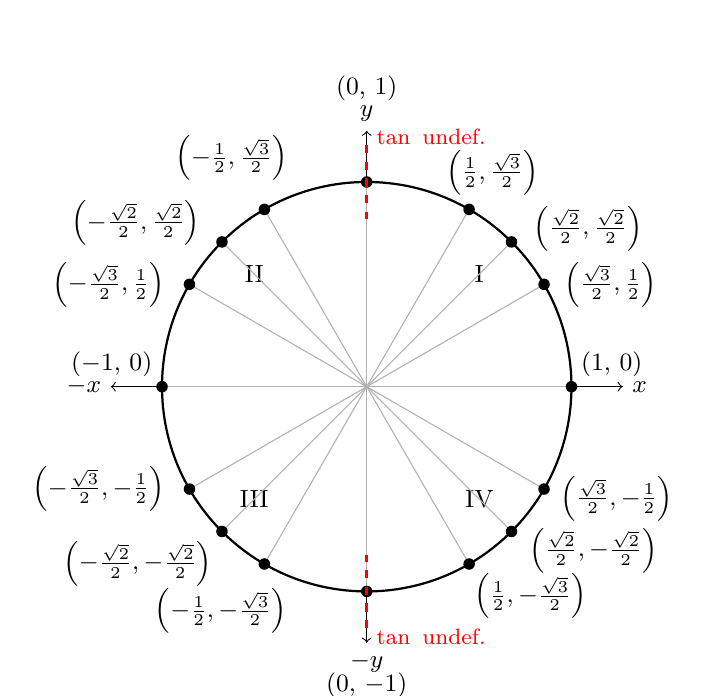
\begin{tikzpicture}[scale=2.6, font=\small]

  % axes
  \draw[->] (-1.25,0) -- (1.25,0) node[right] {\m{x}};
  \draw[->] (1.25,0) -- (-1.25,0) node[left] {\m{-x} };

  \draw[->] (0,1.25) -- (0,-1.25) node[below] {\m{-y}};
  \draw[->] (0,-1.25) -- (0,1.25) node[above] {\m{y}};

  % unit circle
  \draw[thick] (0,0) circle(1);

  % quadrant labels
  \node at ( 0.55, 0.55) {\small I};
  \node at (-0.55, 0.55) {\small II};
  \node at (-0.55,-0.55) {\small III};
  \node at ( 0.55,-0.55) {\small IV};

  % ---- standard angles: (angle, x-coord label offset, y-coord label offset) ----
  \foreach \angle/\cx/\cy/\lab in {
      0    / 0.08 / 0.10 / {0},
      30   / 0.10 / 0.10 / {\pi/6},
      45   / 0.08 / 0.10 / {\pi/4},
      60   / 0.04 / 0.12 / {\pi/3},
      90   / 0.00 / 0.12 / {\pi/2},
      120  / 0.00 / 0.12 / {2\pi/3},
      135  / 0.00 / 0.10 / {3\pi/4},
      150  / 0.00 / 0.10 / {5\pi/6},
      180  / 0.00 / 0.10 / {\pi},
      210  / 0.00 / 0.00 / {7\pi/6},
      225  / 0.00 / 0.00 / {5\pi/4},
      240  / 0.00 / 0.00 / {4\pi/3},
      270  / 0.00 / 0.00 / {3\pi/2},
      300  / 0.00 / 0.00 / {5\pi/3},
      315  / 0.00 / 0.00 / {7\pi/4},
      330  / 0.00 / 0.00 / {11\pi/6}
  }{
    \draw[gray!60, thin] (0,0) -- (\angle:1);
    \fill (\angle:1) circle(0.8pt);
  }

  % ---- labelled points (angle : cos, sin) ----
  \node[above right] at ( 0:1)   {\m{(1,\,0)}};
  \node[above right] at ( 20:1)   {\m{\!\left(\tfrac{\sqrt3}{2},\tfrac{1}{2}\right)}}; %Angle is 30, but moving them down for visibility purposes
  \node[above right] at ( 38:1)   {\m{\!\left(\tfrac{\sqrt2}{2},\tfrac{\sqrt2}{2}\right)}};
  \node[above left]  at ( 45:1.255)   {\m{\!\left(\tfrac{1}{2},\tfrac{\sqrt3}{2}\right)}};
  \node[above]       at ( 90:1.35)   {\m{(0,\,1)}};
  \node[above right] at (135:1.356)   {\m{\!\left(-\tfrac{1}{2},\tfrac{\sqrt3}{2}\right)}};
  \node[above left]  at (140:1)   {\m{\!\left(-\tfrac{\sqrt2}{2},\tfrac{\sqrt2}{2}\right)}};
  \node[above left]  at (160:1)   {\m{\!\left(-\tfrac{\sqrt3}{2},\tfrac{1}{2}\right)}};
  \node[above left]  at (180:1)   {\m{(-1,\,0)}};
  \node[below left]  at (200:1)   {\m{\!\left(-\tfrac{\sqrt3}{2},-\tfrac{1}{2}\right)}};
  \node[below left]  at (225:1)   {\m{\!\left(-\tfrac{\sqrt2}{2},-\tfrac{\sqrt2}{2}\right)}};
  \node[below left]  at (250:1)   {\m{\!\left(-\tfrac{1}{2},-\tfrac{\sqrt3}{2}\right)}};
  \node[below]       at (270:1.35)   {\m{(0,\,-1)}};
  \node[below right] at (300:1)   {\m{\!\left(\tfrac{1}{2},-\tfrac{\sqrt3}{2}\right)}};
  \node[below right] at (320:1)   {\m{\!\left(\tfrac{\sqrt2}{2},-\tfrac{\sqrt2}{2}\right)}};
  \node[below right] at (337:1)   {\m{\!\left(\tfrac{\sqrt3}{2},-\tfrac{1}{2}\right)}};

  % ---- tan undefined markers ----
  \draw[red, very thick, dashed]
      (90:1.18)  -- (90:0.82)
      (270:1.18) -- (270:0.82);
  \node[red, right, font=\footnotesize] at (90:1.22)
      {\m{\tan\text{ undef.}}};
  \node[red, right, font=\footnotesize] at (270:1.22)
      {\m{\tan\text{ undef.}}};

\end{tikzpicture}
\end{center}

\medskip

\noindent\textbf{Why \m{\tan x} causes problems at \m{x = \pm\pi/2}.}\quad
Since \m{\tan x = \sin x / \cos x}, the function is undefined wherever \m{\cos x = 0}, namely at
\m{x = \pm\tfrac{\pi}{2},\, \pm\tfrac{3\pi}{2}, \ldots} On the unit circle these correspond to the
points \m{(0, 1)} and \m{(0, -1)} where the \m{x}-coordinate (i.e.\ \m{\cos x}) is zero.

\medskip

For an ODE such as \m{y'' + (\tan x)\,y = e^x}, the coefficient \m{\tan x} is
\textbf{continuous on any open interval not containing these points}. The largest such interval
centered at \m{x = 0} is therefore \m{\left(-\dfrac{\pi}{2},\, \dfrac{\pi}{2}\right)}, which is
exactly the interval guaranteed by the existence and uniqueness theorem.

\medskip

\begin{center}
\renewcommand{\arraystretch}{1.4}
\begin{tabular}{lll}
\hline
\textbf{Function} & \textbf{Undefined at} & \textbf{Continuous on} \\
\hline
\m{\tan x = \sin x / \cos x}   & \m{x = \tfrac{\pi}{2} + n\pi}  & each \m{\left(-\tfrac{\pi}{2}+n\pi,\, \tfrac{\pi}{2}+n\pi\right)} \\
\m{\cot x = \cos x / \sin x}   & \m{x = n\pi}                   & each \m{(n\pi,\,(n+1)\pi)} \\
\m{\sec x = 1/\cos x}          & \m{x = \tfrac{\pi}{2} + n\pi}  & same as \m{\tan x} \\
\m{\csc x = 1/\sin x}          & \m{x = n\pi}                   & same as \m{\cot x} \\
\hline
\multicolumn{3}{l}{\small \m{n \in \mathbb{Z}}}
\end{tabular}
\end{center}


% ============================================================
% SECTION 1 (LESSON 12) — VARIATION OF PARAMETERS
% ============================================================
\section{Variation Of Paramters}

\subsection{Application to linear nth-order systems }

    \subsubsection{Application to Linear 1st order systems}
    \subsubsection{Application to Linear 2nd order systems}
\subsection{Introduction of Integral-Defined Functions}
\subsection{Discussing the Role of The Constant of Integration}

% ============================================================
% SECTION 2 (LESSON 13) — CAUCHY - EULER EQUATIONS
% ============================================================
\section{Cauchy-Euler Equations}

\subsection{ }

    \subsubsection{General Form and Terminology}


% ============================================================
% SECTION 3 (LESSON 14) — SPRING - MASS SYSTEMS
% ============================================================
\section{Spring - Mass Systems}

\subsection{Introduction to Higher Order Linear ODEs}

    \subsubsection{General Form and Terminology}

% ============================================================
% SECTION 4 (LESSON 15) — POWER SERIES SOLUTIONS
% ============================================================
\section{Power Series Solutions}

\subsection{Introduction to Higher Order Linear ODEs}

    \subsubsection{General Form and Terminology}
    
% ============================================================
% PRACTICE PROBLEMS
% ============================================================
\newpage
\section*{Practice Problems}
\addcontentsline{toc}{section}{Practice Problems}
\addcontentsline{toc}{subsection}{4.6 Homework}
\addcontentsline{toc}{subsection}{4.7 Homework}
\addcontentsline{toc}{subsection}{5.1 Homework}
\addcontentsline{toc}{subsection}{6.1 Homework}

One problem of each exam type from Unit 02. Work through these at the end.

\bigskip
\hrule
\bigskip

\noindent\textbf{P1.}\quad\textit{Existence \& Uniqueness --- Interval of Solution}\\
Find the largest interval centered about \m{x = 0} on which the IVP has a unique solution.
\[
    y'' + (\tan x)\,y = e^x, \qquad y(0) = 1,\quad y'(0) = 0.
\]
\annotspace[5cm]

\hrule\medskip

\noindent\textbf{P2.}\quad\textit{Wronskian and Fundamental Set Verification}\\
Verify that \m{y_1 = x^2} and \m{y_2 = x^4} form a fundamental set of solutions of
\m{x^2 y'' - 5xy' + 8y = 0} on \m{(0,\infty)} by computing \m{W(x^2, x^4)}.
\annotspace[5.5cm]

\hrule\medskip

\noindent\textbf{P3.}\quad\textit{Reduction of Order}\\
Given that \m{y_1 = x^2} solves \m{x^2 y'' + 2xy' - 6y = 0}, use reduction of order to find a
second solution \m{y_2(x)}.
\annotspace[6cm]

\hrule\medskip

\noindent\textbf{P4.}\quad\textit{Characteristic Equation --- Repeated Root (IVP)}\\
Solve the initial value problem.
\[
    y''' + 6y'' + 9y' = 0, \qquad y(0) = 0,\quad y'(0) = 1,\quad y''(0) = -4.
\]
\annotspace[6cm]

\hrule\medskip

\noindent\textbf{P5.}\quad\textit{Characteristic Equation --- Higher Order}\\
Find the general solution of
\[
    \frac{d^4y}{dx^4} - 14\,\frac{d^2y}{dx^2} - 32y = 0.
\]
\annotspace[5.5cm]

\hrule\medskip

\noindent\textbf{P6.}\quad\textit{Undetermined Coefficients --- Superposition with Modification Rule (IVP)}\\
Solve the initial value problem.
\[
    y'' + 4y' + 4y = (7 + x)e^{-2x}, \qquad y(0) = 6,\quad y'(0) = 8.
\]
\annotspace[6cm]

\hrule\medskip

\noindent\textbf{P7.}\quad\textit{Undetermined Coefficients --- Resonance (IVP)}\\
Solve the initial value problem.
\[
    y'' + y = 10\cos(2x) - 4\sin(x), \qquad
    y\!\left(\tfrac{\pi}{2}\right) = -1,\quad y'\!\left(\tfrac{\pi}{2}\right) = 0.
\]
\annotspace[6cm]

\hrule\medskip

\noindent\textbf{P8.}\quad\textit{Annihilator --- Identify the Operator}\\
Find a linear differential operator that annihilates each function.
\begin{align*}
    \text{(a)}\quad &(7 - e^x)^2 \\[4pt]
    \text{(b)}\quad &8 + e^x\cos(5x) \\[4pt]
    \text{(c)}\quad &e^{-x}\sin(x) - e^{7x}\cos(x)
\end{align*}
\annotspace[5.5cm]

\hrule\medskip

\noindent\textbf{P9.}\quad\textit{Annihilator --- Full Solution}\\
Use the annihilator method to find the general solution of
\[
    y'' + 3y' - 4y = 16e^{2x}.
\]
\annotspace[6cm]

\hrule\medskip

\noindent\textbf{P10.}\quad\textit{Mixed Review --- Third-Order Equation}\\
Find the general solution of
\[
    3y''' + 7y'' + 10y' + 8y = 0.
\]
\textit{Hint: test \m{r = -4/3}.}
\annotspace[8cm]

\end{document}